\documentclass[12pt,a4paper]{article}
% Page parameters
\usepackage[
left=3cm,
right=2cm,
top=2cm,
bottom=2cm,
bindingoffset=0cm]{geometry}
% Lines interval
\renewcommand\baselinestretch{1.25}
% Fonts
%\usepackage{cmlgc}
%
\usepackage[T2A]{fontenc}
\usepackage[utf8]{inputenc}
%\usepackage{biblatex}
\usepackage{indentfirst}
\usepackage{amssymb,amsmath}
\usepackage{empheq}
\usepackage{graphicx}
\usepackage{enumerate}
\usepackage{hyperref}
%\usepackage{appendix}
%\usepackage{doi}
\usepackage[space]{cite}
%

% Colors
%\usepackage{color}
%\usepackage[usenames,dvipsnames,svgnames,table]{xcolor}

% Custom commands
\usepackage{common_math}
\newcommand{\todo}[1]{\textcolor{red}{#1}}

% Section style (Dot after arabic numer).
%\usepackage{titlesec}
%\titlelabel{\thetitle.\quad}

% Dots in Table Of contents.
%\usepackage[subfigure]{tocloft}
%\renewcommand{\cftsecleader}{\cftdotfill{\cftdotsep}}

% Equation numeration
\numberwithin{equation}{section}
%\numberwithin{equation}{subsection}
%\numberwithin{equation}{subsubsection}

\title{}
\begin{document}
\section{Introduction}

Ef is a software for charged particles dynamics simulation.  It's
primary areas of application are accelerator science and plasma
physics.

Ef focuses on nonrelativistic energies. Currently, particular
emphasis is placed on low-energy beams, such that can be found in ion
sources and electron guns.

Particles dynamics is traced under action of external electromagnetic
fields.  Particle self-interaction is taken into account with
\href{https://en.wikipedia.org/wiki/Particle-in-cell}{particle-in-cell} 
method.

Attention is given to integration with CAD software to allow for
simulation of complex real-life experimental setups.  An experimental
plugin for \href{http://www.freecadweb.org/}{FreeCAD} exists.

Ef is a free software -- it's source code is open and avaible for
modification and redistribution.  It is written mostly in C++.  Basic
MPI support allows to take advantage of parallel execution in
multiprocessor environment.

\href{https://github.com/epicf/epicf/wiki/1-Rationale-and-Aims}{Development goals}
and 
\href{https://github.com/epicf/epicf/wiki/3-Feature-Matrix-and-Development-Roadmap}{current features}
are described in detail in appropriate wiki sections,
as well as \href{https://github.com/epicf/epicf/wiki/4-Installation}{installation procedure}.
Some usage \href{https://github.com/epicf/epicf/wiki/Examples}{examples}
are also given.

%%% Local Variables:
%%% mode: latex
%%% TeX-master: "ef"
%%% End:

\section{Conduction sphere potential}
Currently epicf is not capable to load any external electic fields or
use any analytic expressions for them.  However, it is possible to
specify geometric primitives (such as sphere, cube, etc.) inside
computation domain, that will act like conductors with fixed
potential. To some extent, this allows to produce desired field
destribution.

In this example, numerically calculated potential of charged
conducting sphere is compared with analytical expression.

Potential of a charged conducting sphere with radius R is constant
inside the sphere and equals to point charge potential outside the
sphere:
\begin{gather}
  \varphi( \mathbf{r} )
  = 
  \begin{cases}
    \varphi_0, \,\, r \le R \\
    \dfrac{R}{r} \varphi_0, \,\, r > R
  \end{cases}
\end{gather}

In config file, definition of such sphere is done inside
\texttt{[Inner\_region\_sphere]} section.

\begin{verbatim}
    [Inner_region_sphere.sphere]
    potential = 3.0
    sphere_origin_x = 5.0
    sphere_origin_y = 5.0
    sphere_origin_z = 5.0
    sphere_radius = 0.5
\end{verbatim}

Since we don't want any particles, there is no need to specify
sources.

Currently, there is no option in Epicf to calculate fields only - the
program will attempt to evaluate several dynamics time steps. To
mitigate such effect, it is possible to set saving time step greter
than total simulation time:

[code]

When analysing results, it is possible to plot 2d potential
distribution similar to previous example.  

[pics]

More illustrative is plot along axis passing though a center of the
sphere:

\begin{figure}[H]
  \centering
  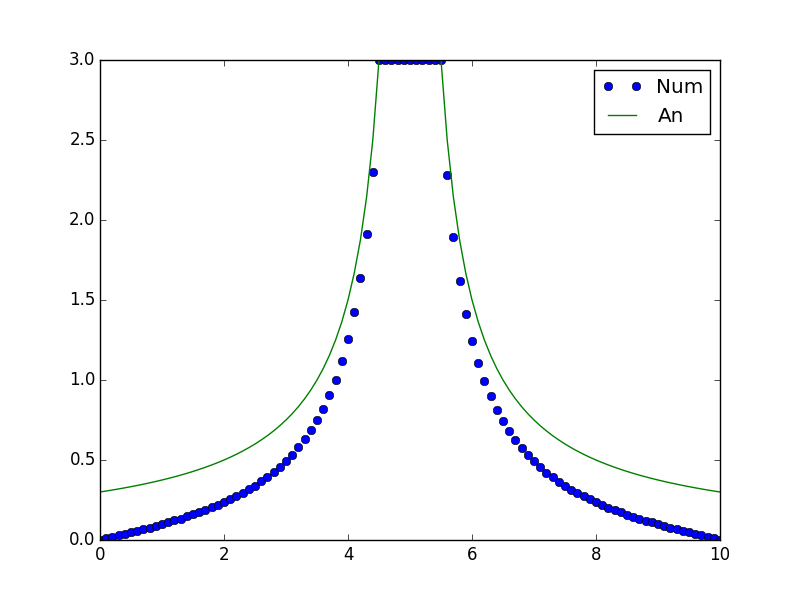
\includegraphics[scale=0.5]{./figs/ex4_conducting_sphere_potential/potential_along_z.png}
  \caption{Comparison of numerical and analytical results for
    conducting sphere potential}
\end{figure}

It can be seen, that agreement is not very good. This can be related
to the fact, that in the simulation potentials on boundaries of
computation domain are set to zero. In reality potential potential
slowly approaches zero as distance from the sphere increases.

%%% Local Variables:
%%% mode: latex
%%% TeX-master: "ef"
%%% End:

%\appendix
%\include{appendixA}
\bibliographystyle{plainurl}
\bibliography{bib}{}


%%%%%%%%


\end{document}
